\section{Optimisation des hyper-paramètres et choix d'un modèle}\label{chapter-ML-section-hyperparameters}
Le choix d'un modèle et de ses hyper-paramètres est l'objet de cette section.
Deux types de modèle sont étudiés:
\begin{itemize}
\item des arbres de décision améliorés, introduits section~\ref{chapter-ML-section-XGB}, notés XGB;
\item des réseaux de neurones profonds, introduits section~\ref{chapter-ML-section-DNN}, notés DNN.
\end{itemize}
\par
Les hyper-paramètres des XGBs sont:
\begin{itemize}
\item la profondeur maximale des arbres \MaxDepth;
\item la quantité d'échantillons minimale dans une branche \MinChildWeight;
\item le nombre d'arbres \Nestimators;
\item le gain minimal $\gamma$;
\item le taux d'apprentissage $\eta$;
\item la fonction de coût \Loss;
\item la liste des variables d'entrée.
\end{itemize}
Les hyper-paramètres des DNNs sont:
\begin{itemize}
\item le nombre de couches cachées $N_L$;
\item le nombre de neurones par couche cachée $N_N$;
\item la fonction d'activation des neurones des couches cachées;
\item la méthode d'optimisation;
\item la fonction de coût \Loss;
\item le mode d'initiation des poids;
\item la liste des variables d'entrée.
\end{itemize}
\par
Il est difficile de définir un seul score quantifiant la qualité d'un modèle.
Plusieurs métriques sont considérées afin d'évaluer les modèles:
\begin{itemize}
\item les valeurs de
\LossMSE,
\LossMAE,
\LossMAPE;
\item la résolution relative des modèles,
ou \og largeur à $1\sigma$ \fg,
notée \OneSigmaWidth,
estimée par
la moyenne
de
la largeur du premier quantile de la distribution de la réponse $r$ des modèles
sur des intervalles de \SI{10}{\GeV} sur $\ytrue=m_{\higgsML}$,
où la réponse $r$ est définie comme
\begin{equation}
r = \frac{\ypred}{\ytrue} = \frac{F(\vec{x})}{m_{\higgsML}}
\mend[,]
\end{equation}
\ie
\begin{equation}
\OneSigmaWidth = \Average{\eval{\sigma\left(\frac{\ypred}{\ytrue}\right)}_{\ytrue\in [n, n+1]\times\SI{10}{\GeV}}}_n
\mend
\end{equation}
\end{itemize}
Pour toutes ces métriques, l'objectif est la plus petite valeur possible.
De plus, quatre domaines de masse sont définis:
\begin{itemize}
\item basse masse : $m_{\higgsML} < \SI{150}{\GeV}$, incluant en particulier les bosons \Zboson\ et \higgs;
\item masse moyenne : $\SI{150}{\GeV} \geq m_{\higgsML} < \SI{500}{\GeV}$;
\item haute masse : $m_{\higgsML} \geq \SI{500}{\GeV}$;
\item toute masse : aucune restriction sur $m_{\higgsML}$.
\end{itemize}
Ils permettent de comparer les performances des modèles sur certaines gammes de masse uniquement.
Sauf contre-indication, toute la gamme de masse est considérée.
\subsection{Variables d'entrée}
Les différentes variables d'entrée considérées sont listées dans la section~\ref{chapter-ML-section-evt_gen-inputs}.
La plupart de celles-ci sont généralement déjà exploitées dans les analyses en cours.
Ce n'est toutefois pas garanti, en particulier pour les variables relatives à l'activité hadronique additionnelle.
L'utilisation de variables supplémentaires demande,
en plus de la mise en place de leur obtention,
de reprendre potentiellement de longues étapes de calculs.
Se restreindre à un sous-ensemble des variables d'entrée,
si cela ne dégrade pas la qualité des modèles,
pourrait donc faciliter l'intégration de nos modèles.
\par
Les sous-ensembles des variables d'entrée sont définis par les restrictions suivantes:
\begin{itemize}
\item sans \Npu: la variable \Npu\ n'est pas utilisée;
\item sans \Nnu: la variable \Nnu\ n'est pas utilisée;
\item sans AHA: les variables d'activité hadronique additionnelle ne sont pas utilisées;
\item sans jets: les variables relatives aux jets (dont AHA) ne sont pas utilisées;
\item sans \mT: les masses transverses ne sont pas utilisées;
\item sans METcov: la matrice de covariance de \MET\ n'est pas utilisée.
\end{itemize}
L'application de plusieurs de ces restrictions est également testée.
\par
Les performances modèles entraînés avec les différents ensembles de variables d'entrée sont données
figure~\ref{fig-XGB_inputs} pour les XGBs
et
figure~\ref{fig-DNN_inputs}
pour les DNNs.
Les modèles concernés par plusieurs restrictions sont comptés de manière pondérée dans chaque groupe correspondant à une restriction unique.
Par exemple, un modèle soumis à la restriction \og sans \Npu\ \fg{} et \og sans \Nnu\ \fg{} a un poids de $\frac{1}{2}$ dans chacun de ces deux groupes.
Une pondération par la quantité de modèles dans chaque groupe est de plus appliquée pour supprimer le biais lié à la quantité accrue de modèles dans le groupe sans restrictions.
Les histogrammes ainsi créés sont superposés.
Il est alors possible de voir les contributions de chacune des restrictions aux valeurs obtenues sur la métrique d'évaluation illustrée.
\begin{figure}[h]
\centering

\subcaptionbox{Évaluation par \LossMAPE.\label{subfig-XGB_inputs-mape}}[.45\textwidth]
{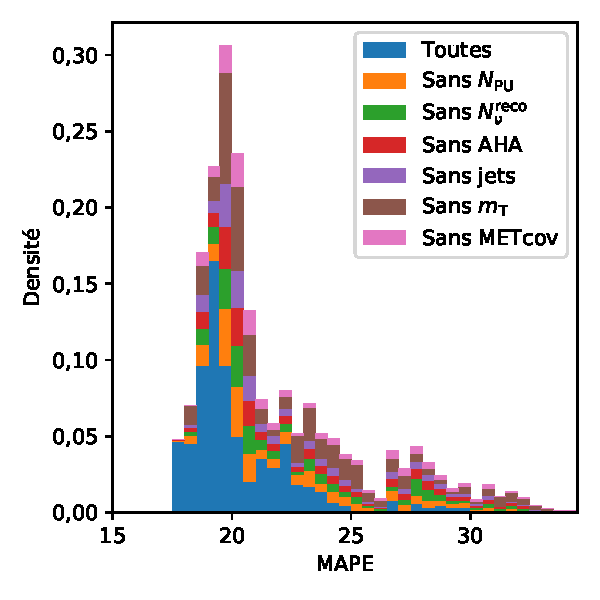
\includegraphics[width=.45\textwidth]{\PhDthesisdir/plots_and_images/my_plots/ML/from_ML_plots/global_comparisons/XGB_inputs_all-full_mape.pdf}\vspace{-\baselineskip}}
\hfill
\subcaptionbox{Évaluation par \OneSigmaWidth.\label{subfig-XGB_inputs-1sigw}}[.45\textwidth]
{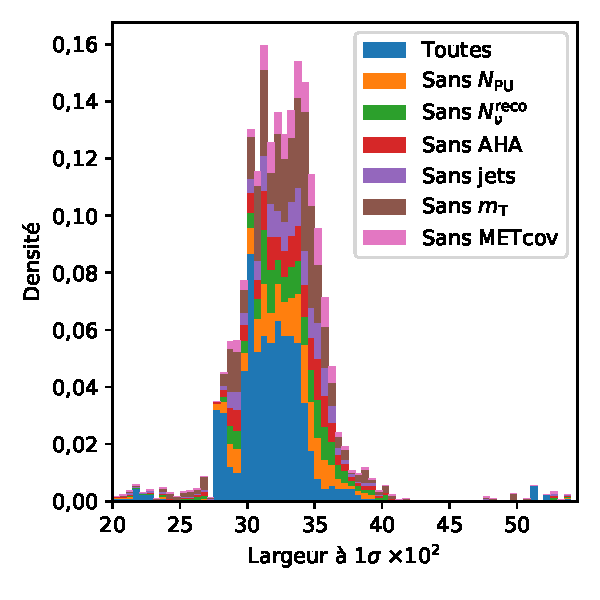
\includegraphics[width=.45\textwidth]{\PhDthesisdir/plots_and_images/my_plots/ML/from_ML_plots/global_comparisons/XGB_inputs_all-full_1sig_width.pdf}\vspace{-\baselineskip}}

\caption{Évaluations des XGBs regroupés selon les variables d'entrée.}
\label{fig-XGB_inputs}
\end{figure}
\begin{figure}[h]
\centering

\subcaptionbox{Évaluation par \LossMAPE.\label{subfig-DNN_inputs-mape}}[.45\textwidth]
{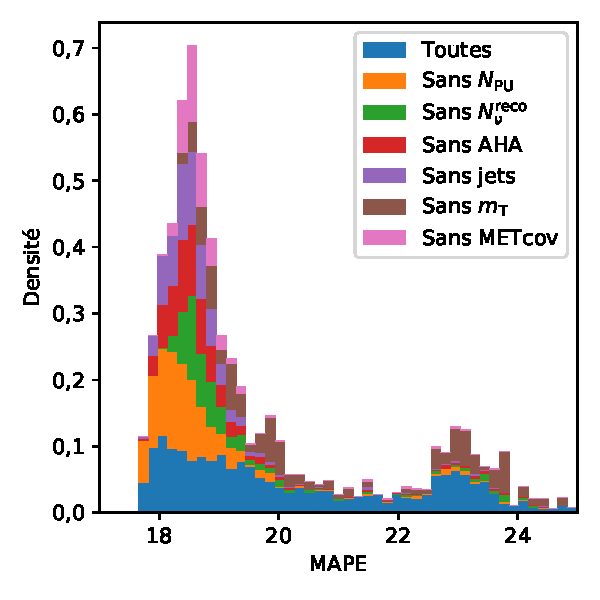
\includegraphics[width=.45\textwidth]{\PhDthesisdir/plots_and_images/my_plots/ML/from_ML_plots/global_comparisons/DNN_inputs_all-full_mape.pdf}\vspace{-\baselineskip}}
\hfill
\subcaptionbox{Évaluation par \OneSigmaWidth.\label{subfig-DNN_inputs-1sigw}}[.45\textwidth]
{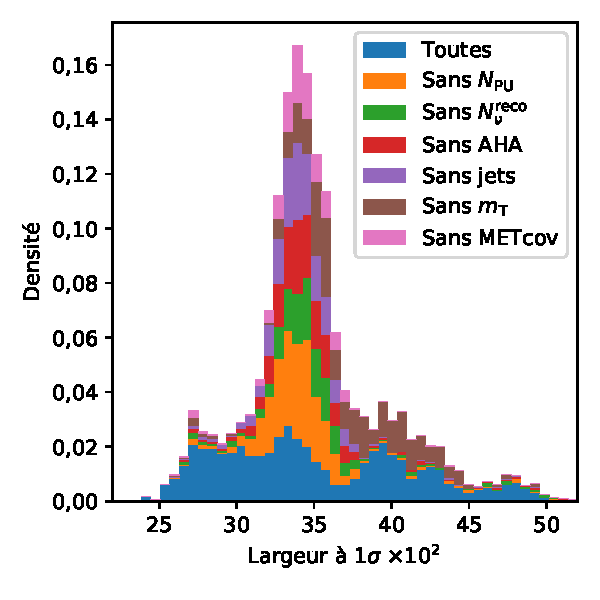
\includegraphics[width=.45\textwidth]{\PhDthesisdir/plots_and_images/my_plots/ML/from_ML_plots/global_comparisons/DNN_inputs_all-full_1sig_width.pdf}\vspace{-\baselineskip}}

\caption{Évaluations des DNNs regroupés selon les variables d'entrée.}
\label{fig-DNN_inputs}
\end{figure}
\par
Dans le cas des XGBs,
l'évaluation des modèles par \LossMAPE, en figure~\ref{subfig-XGB_inputs-mape},
donne des valeurs situées entre \num{17} et \num{35}.
Le cœur de la distribution,
à $\LossMAPE=\num{19}\pm\num{2}$,
est plutôt constitué
de modèles utilisant
toutes les entrées
dans sa partie gauche ($\LossMAPE<\num{19}$)
et
de modèles utilisant
un sous-ensemble d'entrées
dans sa partie droite ($\num{19}<\LossMAPE<\num{22}$).
De plus, les basses valeurs de \LossMAPE, en-dessous de \num{18.5},
sont presque exclusivement obtenues avec des modèles utilisant toutes les entrées.
À l'inverse, la queue à hautes valeurs de la distribution obtenue ($\LossMAPE>\num{23}$) est largement dominée par les contributions des modèles avec un sous-ensemble d'entrées.
\par
La plupart des XGBs ont
une largeur \OneSigmaWidth, en figure~\ref{subfig-XGB_inputs-1sigw},
située entre \num{27} et \num{38}.
Cependant,
les XGBs utilisant toutes les variables d'entrée
exhibent une distribution de \OneSigmaWidth\ légèrement décalée vers de plus faibles valeurs.
\par
Dans le cas des DNNs,
la distribution de la métrique \LossMAPE, en figure~\ref{subfig-DNN_inputs-mape},
contient des valeurs situées entre \num{17.5} et \num{25}.
Les DNNs n'utilisant pas \Nnu\
se situent à $\LossMAPE>\num{18}$.
Cette variable permet aux modèles de différencier les canaux
hadroniques, semi-leptoniques et leptoniques,
dont la séparation est discutée dans la section~\ref{chapter-ML-section-discussion}.
Ceux n'utilisant pas \mT\ présentent également des valeurs de \LossMAPE\ uniquement au-delà de \num{18}.
L'utilisation de ces variables permet donc d'obtenir de meilleurs modèles.
Elles sont de plus facilement obtenues à partir du \emph{dilepton}, défini chapitre~\refChHTT, et de \MET.
Les analyses avec deux leptons tau dans l'état final exploitent déjà ces observables,
leur utilisation par nos modèles est donc à la fois
pertinente, car les scores de \LossMAPE\ obtenus sont meilleurs,
et
sans incidence sur la facilité d'intégration du modèle à l'analyse.
Les DNNs avec $\LossMAPE\lesssim\num{18}$
exploitent presque tous
les variables relatives aux jets, à l'AHA et à la matrice de covariance de \MET.
Ces entrées sont donc vraisemblablement utiles aux DNNs afin de réaliser la régression.
Enfin,
la restriction sur \Npu\
ne semble pas dégrader les performances des DNNs
selon \LossMAPE.
\par
La distribution de
\OneSigmaWidth, en figure~\ref{subfig-DNN_inputs-1sigw},
montre que les modèles utilisant toutes les entrées peuvent se répartir en trois groupes,
aux alentour des valeurs
\num{0.275}, \num{0.335} et \num{0.395}.
À \num{0.39} apparaît également un groupe de modèles entraînés sans \mT.
À \num{0.33} se trouvent la majorité des modèles entraînés avec une restriction des entrées.
Les modèles de ces groupes ont potentiellement minimisé l'utilisation de certaines variables.
Les modèles d'intérêt sont ceux du groupe se situant à $\OneSigmaWidth \simeq \num{0.275}$.
Il s'agit presque exclusivement de modèles utilisant toutes les variables d'entrée.
\par
L'utilisation de toutes les variables listées dans la section~\ref{chapter-ML-section-evt_gen-inputs}
est donc corrélée avec de meilleures performances
selon les métriques
\LossMAPE\
et
\OneSigmaWidth.
Par la suite, seuls les modèles utilisant toutes les variables, au nombre de 27, sont considérés.
\subsection{Type de modèle}
Les figures~\ref{fig-DNN_vs_XGB-mse_mape} et~\ref{fig-DNN_vs_XGB-1sigma}
présentent les distributions des scores de
\LossMSE,
\LossMAPE\
et
\OneSigmaWidth\
pour l'ensemble des DNNs et des XGBs
utilisant toutes les variables d'entrée.
\par
\begin{figure}[h]
\centering

\subcaptionbox{Évaluation par \LossMSE.\label{subfig-DNN_vs_XGB-mse}}[.45\textwidth]
{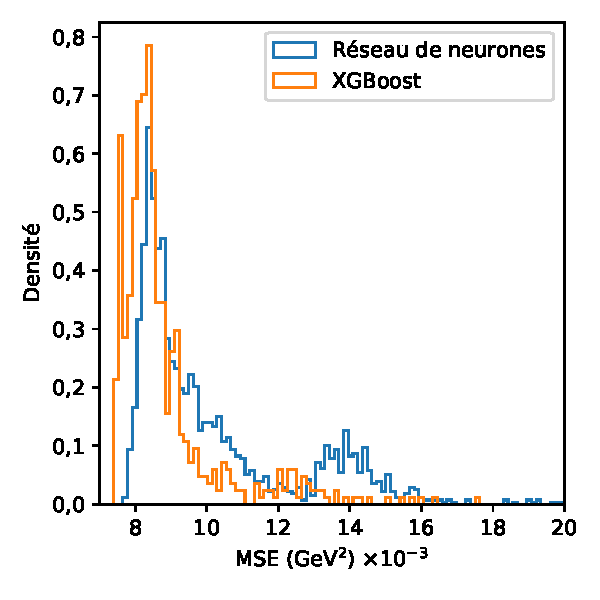
\includegraphics[width=.45\textwidth]{\PhDthesisdir/plots_and_images/my_plots/ML/from_ML_plots/global_comparisons/DNN_vs_XGB_all_inputs-full_mse.pdf}\vspace{-\baselineskip}}
\hfill
\subcaptionbox{Évaluation par \LossMAPE.\label{subfig-DNN_vs_XGB-mape}}[.45\textwidth]
{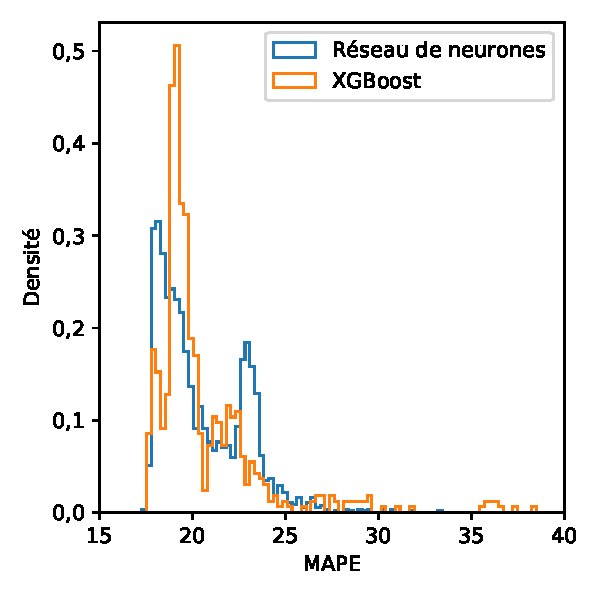
\includegraphics[width=.45\textwidth]{\PhDthesisdir/plots_and_images/my_plots/ML/from_ML_plots/global_comparisons/DNN_vs_XGB_all_inputs-full_mape.pdf}\vspace{-\baselineskip}}

\caption{Évaluations des XGBs et des DNNs par \LossMSE\ et \LossMAPE.}
\label{fig-DNN_vs_XGB-mse_mape}
\end{figure}
\begin{figure}[h]
\centering
%\vspace{\baselineskip}

%\subcaptionbox{\label{subfig-DNN_vs_XGB-mae}}[.45\textwidth]
%{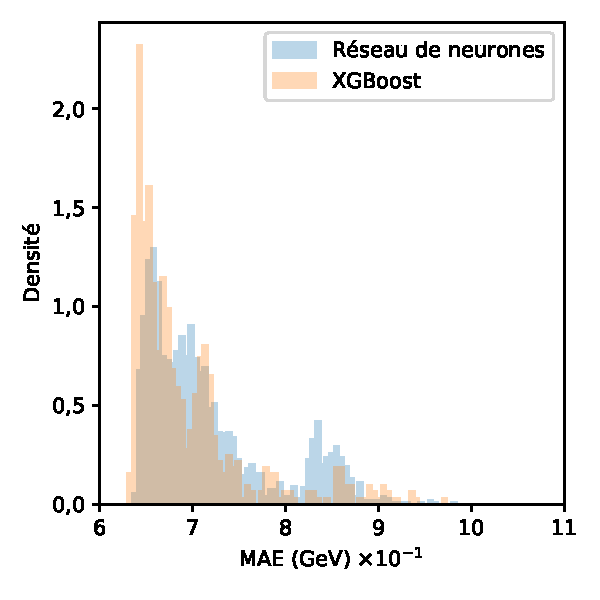
\includegraphics[width=.45\textwidth]{\PhDthesisdir/plots_and_images/my_plots/ML/from_ML_plots/global_comparisons/DNN_vs_XGB_all_inputs-full_mae.pdf}\vspace{-\baselineskip}}
%\hfill
\subcaptionbox{Sur toute la gamme de masse.\label{subfig-DNN_vs_XGB-1sigma}}[.45\textwidth]
{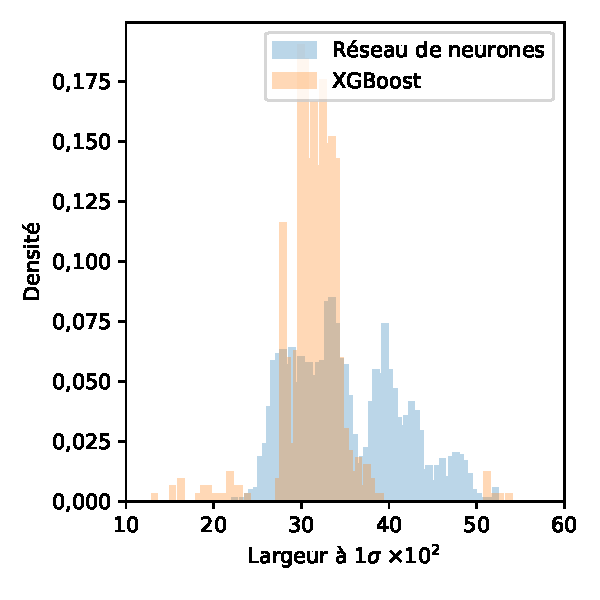
\includegraphics[width=.45\textwidth]{\PhDthesisdir/plots_and_images/my_plots/ML/from_ML_plots/global_comparisons/DNN_vs_XGB_all_inputs-full_1sig_width.pdf}\vspace{-\baselineskip}}
\hfill
\subcaptionbox{À basse masse.\label{subfig-DNN_vs_XGB-low_1sigma}}[.45\textwidth]
{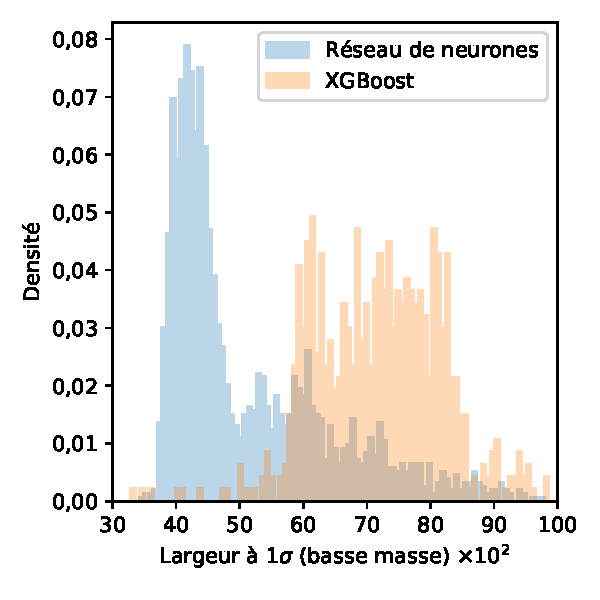
\includegraphics[width=.45\textwidth]{\PhDthesisdir/plots_and_images/my_plots/ML/from_ML_plots/global_comparisons/DNN_vs_XGB_all_inputs-low_1sig_width.pdf}\vspace{-\baselineskip}}

\caption{Évaluations des XGBs et des DNNs par \OneSigmaWidth.}
\label{fig-DNN_vs_XGB-1sigma}
\end{figure}
L'évaluation par \LossMSE, en figure~\ref{subfig-DNN_vs_XGB-mse}, favorise les XGBs.
Le cœur de la distribution de \LossMSE\ pour ces modèles est en effet à \SI{8.1e3}{\GeV^2}
contre \SI{8.5e3}{\GeV^2} pour les DNNs.
En revanche,
l'évaluation par \LossMAPE, en figure~\ref{subfig-DNN_inputs-mape}, favorise les DNNs
avec un groupe de DNNs à $\LossMAPE=\num{18}$
contre \num{19} pour les XGBs.
Un second groupe de DNNs est présent à \num{23}.
\par
La résolution des modèles est évaluée par \OneSigmaWidth\
en figure~\ref{subfig-DNN_vs_XGB-1sigma} pour toute la gamme de masse
et
en figure~\ref{subfig-DNN_vs_XGB-low_1sigma} pour les basses masses.
Sur l'ensemble de la gamme de masse,
les XGBs ont un score de $\num{0.32}\pm\num{0.04}$
et
les DNNs se répartissent en trois groupes
à environ
\num{0.28}, \num{0.33} et \num{0.40}.
%\num{0.275}, \num{0.335} et \num{0.395}.
Les XGBs sont ainsi compétitifs d'après cette évaluation.
Cependant,
les performances des modèles
à basse masse, \ie\ pour $m_{\higgsML} < \SI{150}{\GeV}$,
sont importantes car c'est dans cette gamme de masse que se trouvent les bosons \Zboson\ et \higgs\ du modèle standard.
Sur la figure~\ref{subfig-DNN_vs_XGB-low_1sigma},
l'évaluation à basse masse par \OneSigmaWidth\
les XGBs ont un score de $\num{0.70}\pm\num{0.15}$
alors que les DNNs se répartissent en deux groupes,
le premier à $\num{0.42}\pm\num{0.05}$
et
le second entre $\num{0.50}$ et $\num{1.0}$.
Le premier ensemble de DNNs propose les meilleures résolutions sur les masses des particules du modèle standard.
\par
La réévaluation des modèles par 
\LossMSE\ et \LossMAPE\ à basse masse, en figures~\ref{subfig-DNN_vs_XGB-low_mse} et~\ref{subfig-DNN_vs_XGB-low_mape},
confirme l'obtention de meilleures performances avec les DNNs.
En effet,
les DNNs sont les seuls modèles avec
$\LossMSE < \SI{1.5e3}{\GeV^2}$
et
$\LossMAPE < \num{28}$
à basse masse.
Les XGBs ont des scores de \LossMSE\ et \LossMAPE\ généralement
entre \SI{1.5e3}{\GeV^2} et \SI{4.0e3}{\GeV^2}
et
entre \num{28} et \num{43},
respectivement.
La suite de la sélection d'un modèle est donc faite parmi les DNNs.
\begin{figure}[h]
\centering
%\vspace{\baselineskip}

\subcaptionbox{Évaluation par \LossMSE.\label{subfig-DNN_vs_XGB-low_mse}}[.45\textwidth]
{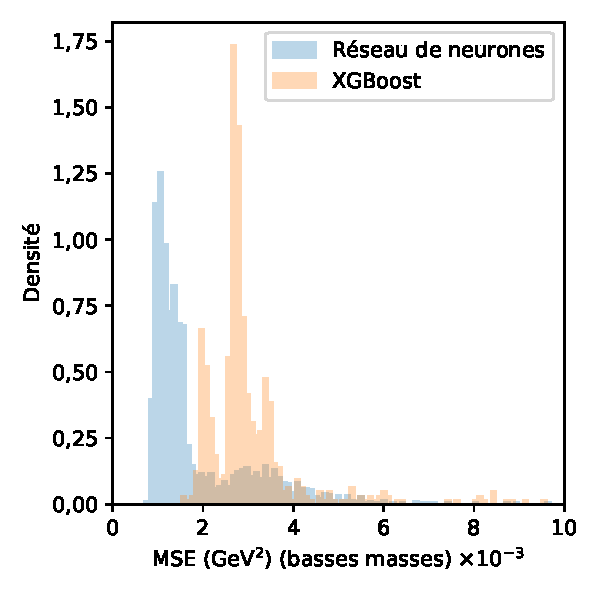
\includegraphics[width=.45\textwidth]{\PhDthesisdir/plots_and_images/my_plots/ML/from_ML_plots/global_comparisons/DNN_vs_XGB_all_inputs-low_mse.pdf}\vspace{-\baselineskip}}
\hfill
\subcaptionbox{Évaluation par \LossMAPE.\label{subfig-DNN_vs_XGB-low_mape}}[.45\textwidth]
{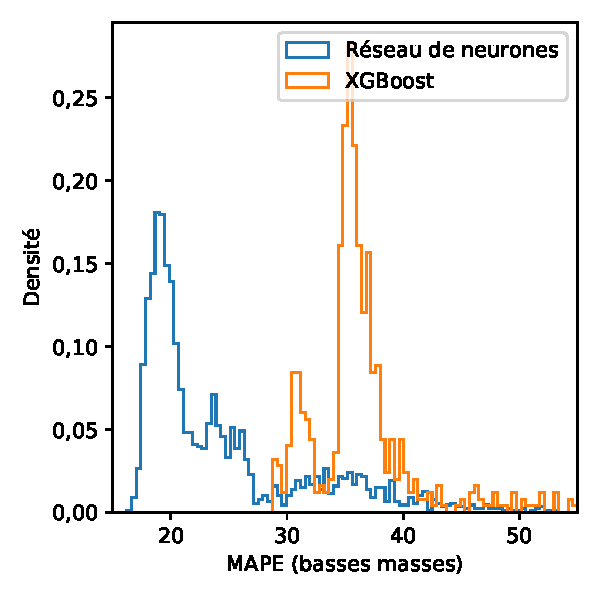
\includegraphics[width=.45\textwidth]{\PhDthesisdir/plots_and_images/my_plots/ML/from_ML_plots/global_comparisons/DNN_vs_XGB_all_inputs-low_mape.pdf}\vspace{-\baselineskip}}

\caption{Évaluations des XGBs et des DNNs par \LossMSE\ et \LossMAPE\ à basse masse.}
\label{fig-DNN_vs_XGB-mse_mape-low}
\end{figure}
\subsection{Fonction de coût}
Les évaluations des DNNs,
regroupés d'après la fonction de coût utilisée lors de leurs entraînements,
selon les métriques
\LossMSE, \LossMAPE, \LossMAE\ et \OneSigmaWidth\
sont représentées sur la figure~\ref{fig-DNN_losses}.
\begin{figure}[h]
\centering

\subcaptionbox{\label{subfig-loss_mse_mape-mse}}[.45\textwidth]
{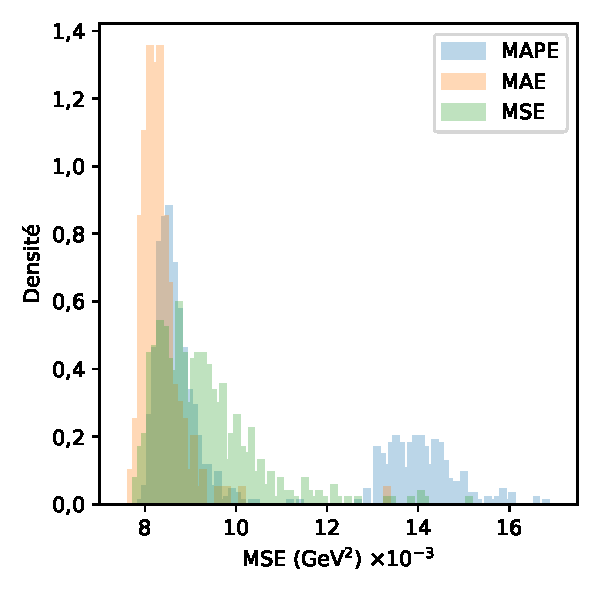
\includegraphics[width=.45\textwidth]{\PhDthesisdir/plots_and_images/my_plots/ML/from_ML_plots/global_comparisons/DNN_loss-full_mse.pdf}\vspace{-\baselineskip}}
\hfill
\subcaptionbox{\label{subfig-loss_mse_mape-mape}}[.45\textwidth]
{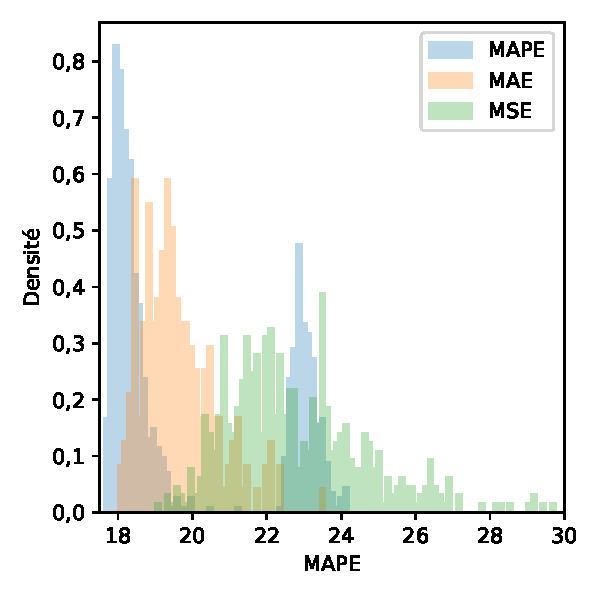
\includegraphics[width=.45\textwidth]{\PhDthesisdir/plots_and_images/my_plots/ML/from_ML_plots/global_comparisons/DNN_loss-full_mape.pdf}\vspace{-\baselineskip}}

\vspace{\baselineskip}

\subcaptionbox{}[.45\textwidth]
{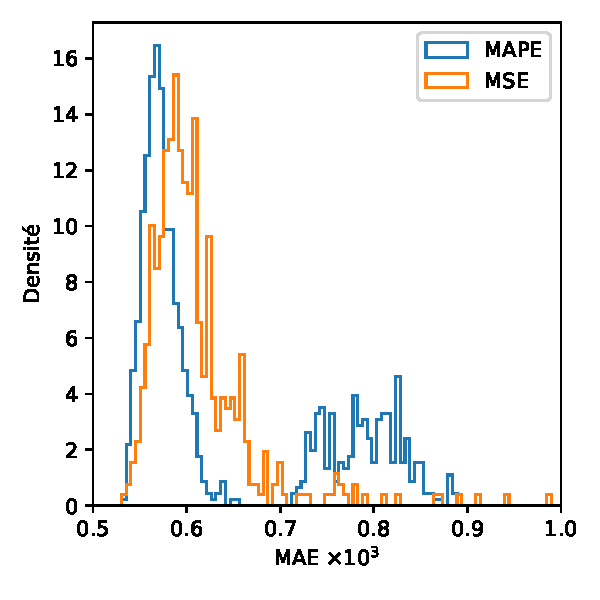
\includegraphics[width=.45\textwidth]{\PhDthesisdir/plots_and_images/my_plots/ML/from_ML_plots/global_comparisons/DNN_loss-full_mae.pdf}\vspace{-\baselineskip}}
\hfill
\subcaptionbox{}[.45\textwidth]
{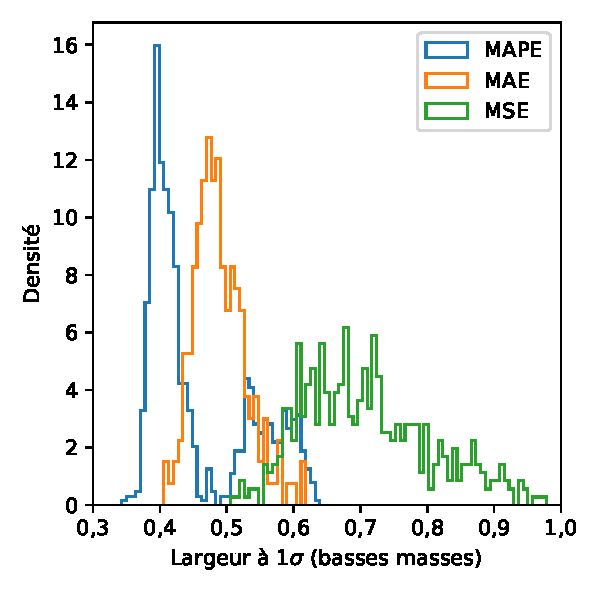
\includegraphics[width=.45\textwidth]{\PhDthesisdir/plots_and_images/my_plots/ML/from_ML_plots/global_comparisons/DNN_loss-low_1sig_width.pdf}\vspace{-\baselineskip}}

\caption{Évaluations des DNNs regroupés selon la fonction de coût par \LossMSE, \LossMAPE, \LossMAE\ et \OneSigmaWidth.}
\label{fig-DNN_losses}
\end{figure}
\par
L'évaluation par \LossMSE, figure~\ref{subfig-loss_mse_mape-mse},
montre que les DNNs entraînés avec $\Loss=\LossMSE$
présentent une score
compris entre \SI{7.5e3}{\GeV^2} et \SI{15e3}{\GeV^2},
la majorité d'entre eux se trouvant en-dessous de \SI{11e3}{\GeV^2}.
Les DNNs entraînés avec $\Loss=\LossMAPE$ en revanche
se séparent en deux groupes.
Le premier se situe entre \SI{7.5e3}{\GeV^2} et \SI{10e3}{\GeV^2},
le second  entre \num{13} et \SI{16e3}{\GeV^2}.

\todo{Models with MAE to be trained}

\subsection{Algorithme d'optimisation et initiation des paramètres}
Trois algorithmes d'optimisation ont été considérés, SGD, Adadelta et Adam.

\todo{QGD complètement dans les choux}

Il apparaît sur la figure~\ref{fig-optimizer} qu'Adam propose de meilleurs modèles qu'Adadelta.
L'initiation des paramètres des neurones n'a en revanche que peu d'influence sur \LossMAPE, comme cela se voit figure~\ref{fig-w_init_mode}.
\begin{figure}[h]
\centering

\subcaptionbox{}[.45\textwidth]
{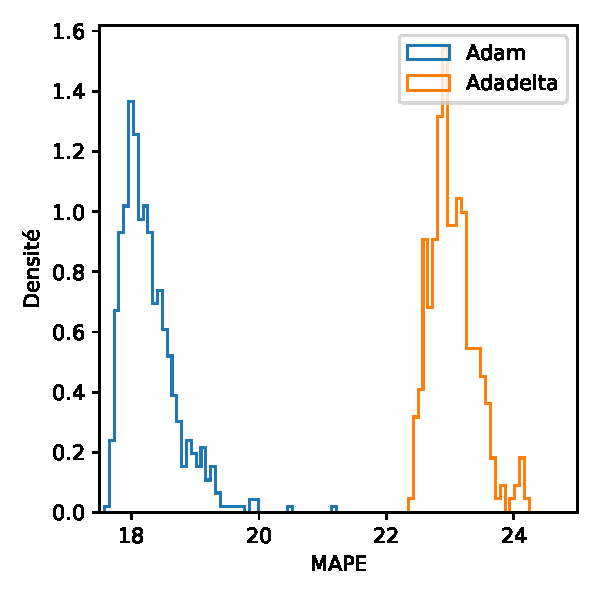
\includegraphics[width=.45\textwidth]{\PhDthesisdir/plots_and_images/my_plots/ML/from_ML_plots/global_comparisons/DNN_optimizer-full_mape.pdf}\vspace{-\baselineskip}}
\hfill
\subcaptionbox{}[.45\textwidth]
{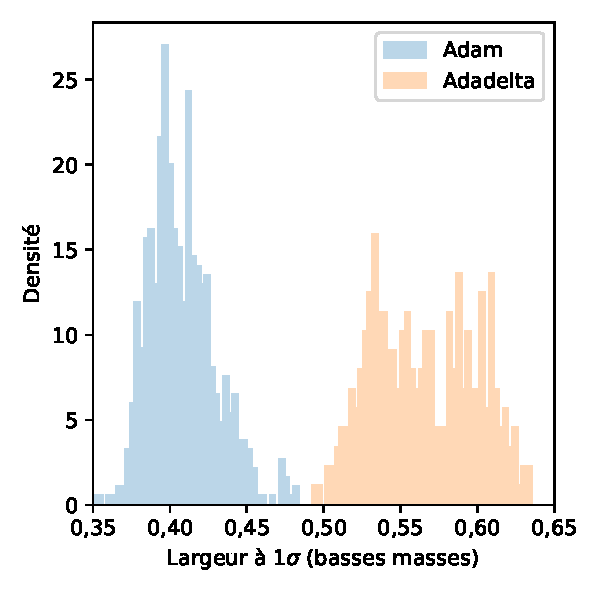
\includegraphics[width=.45\textwidth]{\PhDthesisdir/plots_and_images/my_plots/ML/from_ML_plots/global_comparisons/DNN_optimizer-low_1sig_width.pdf}\vspace{-\baselineskip}}
\caption{Comparaisons des algorithmes d'optimisation.}
\label{fig-optimizer}
\end{figure}
\begin{figure}[h]
\centering
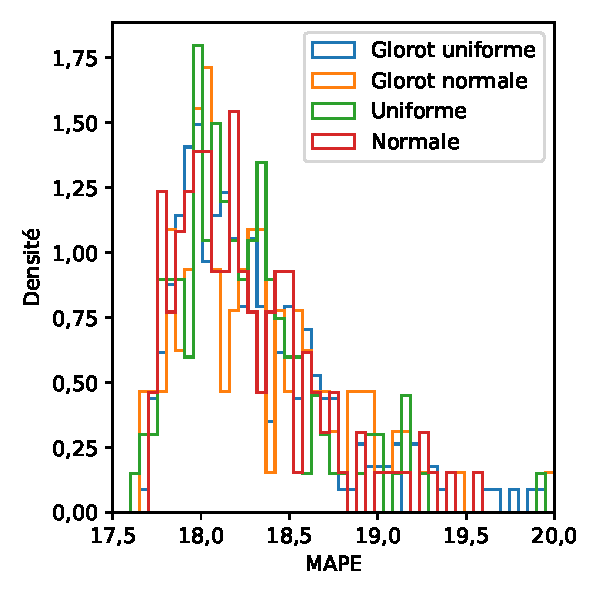
\includegraphics[width=.45\textwidth]{\PhDthesisdir/plots_and_images/my_plots/ML/from_ML_plots/global_comparisons/DNN_w_init_mode-full_mape.pdf}
\caption{Comparaisons des initiations des paramètres.}
\label{fig-w_init_mode}
\end{figure}
\subsection{Structure}
which structure ?

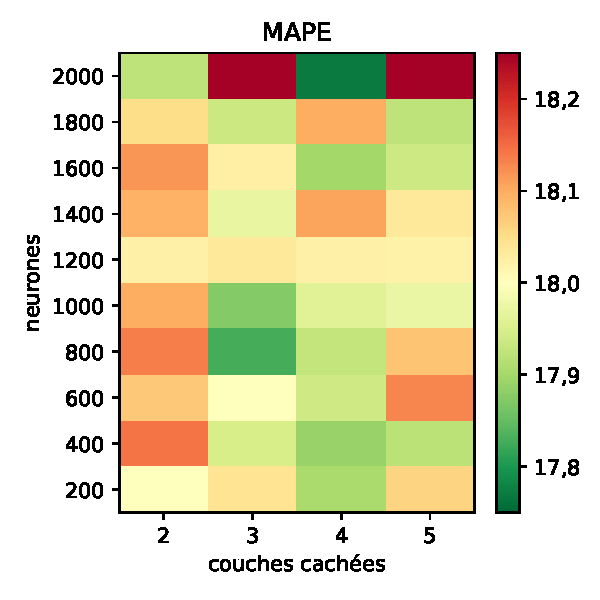
\includegraphics[width=.45\textwidth]{\PhDthesisdir/plots_and_images/my_plots/ML/from_ML_plots/global_comparisons/DNN_structures_reduced-full_mape.pdf}
%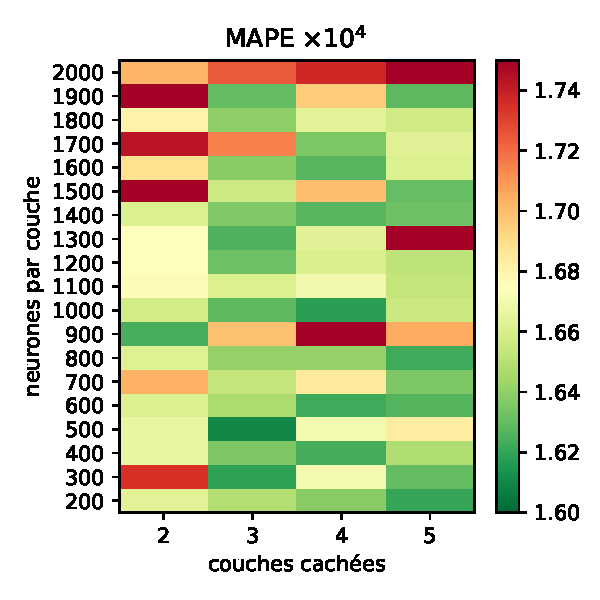
\includegraphics[width=.45\textwidth]{\PhDthesisdir/plots_and_images/my_plots/ML/from_ML_plots/global_comparisons/DNN_structures_all-full_mape.pdf}

several possibilities, but the loss mass region contains the Z boson and is important

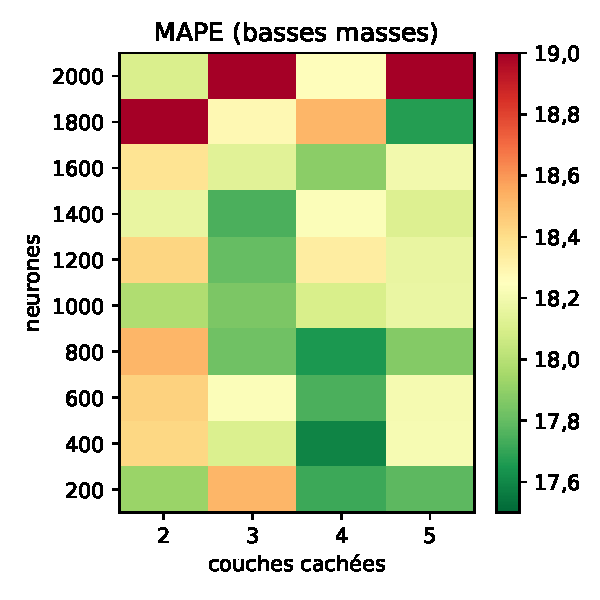
\includegraphics[width=.45\textwidth]{\PhDthesisdir/plots_and_images/my_plots/ML/from_ML_plots/global_comparisons/DNN_structures_reduced-low_mape.pdf}
%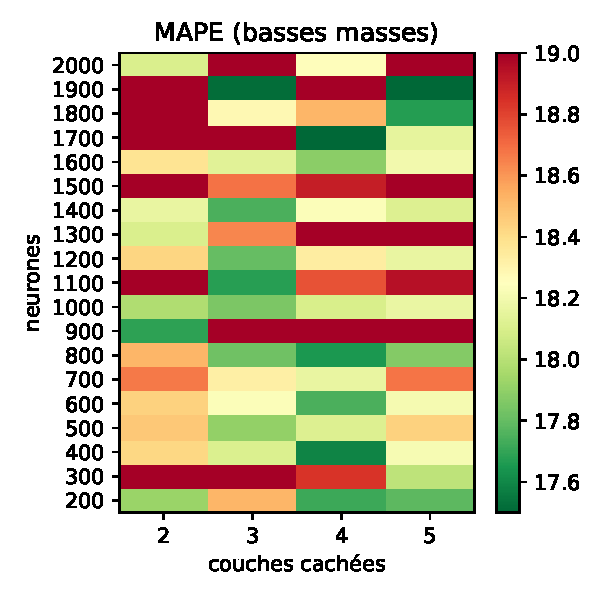
\includegraphics[width=.45\textwidth]{\PhDthesisdir/plots_and_images/my_plots/ML/from_ML_plots/global_comparisons/DNN_structures_all-low_mape.pdf}

2x900 and 5x600 seem to be the best options, check the low mass resolution

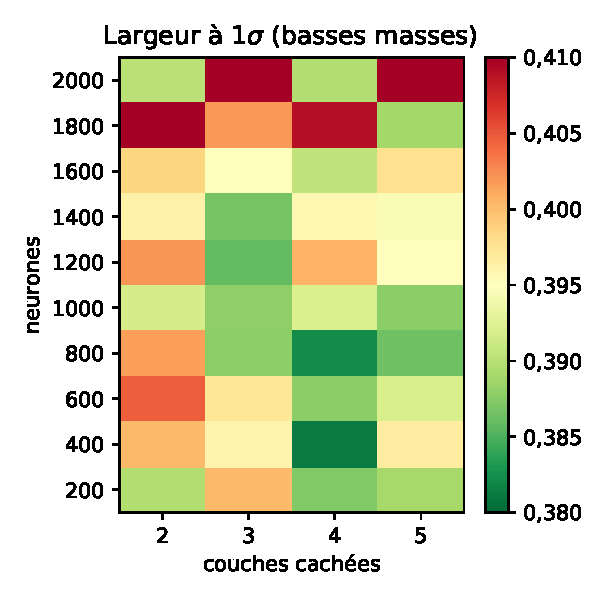
\includegraphics[width=.45\textwidth]{\PhDthesisdir/plots_and_images/my_plots/ML/from_ML_plots/global_comparisons/DNN_structures_reduced-low_1sig_width.pdf}
%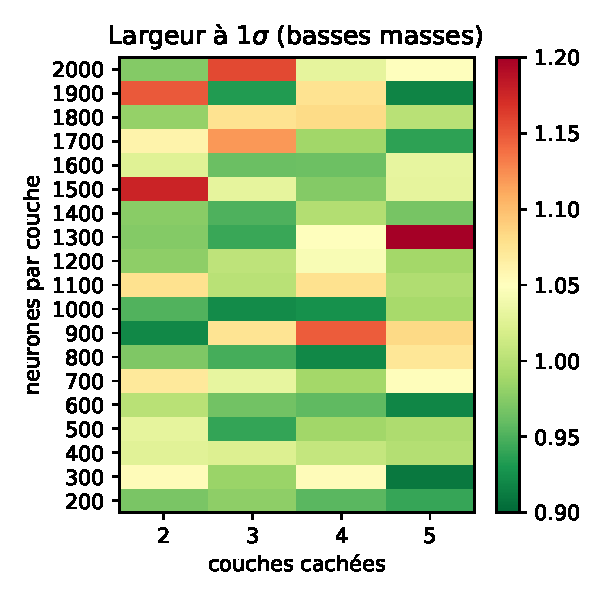
\includegraphics[width=.45\textwidth]{\PhDthesisdir/plots_and_images/my_plots/ML/from_ML_plots/global_comparisons/DNN_structures_all-low_1sig_width.pdf}

5x600 seems good, check the low mass \textbf{calibrated} resolution

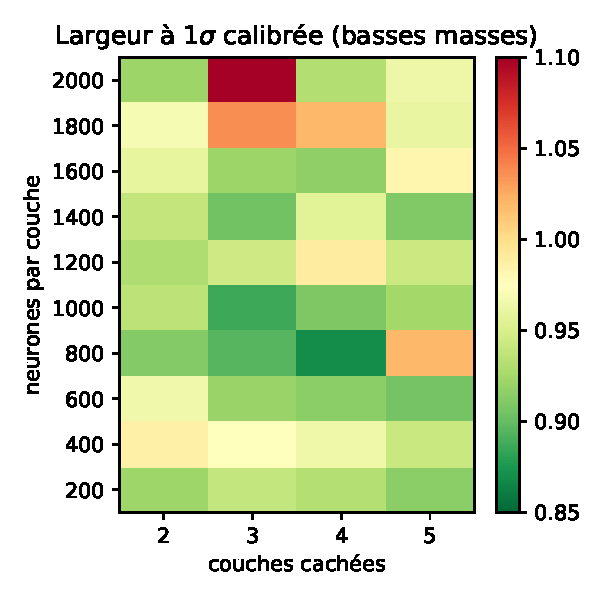
\includegraphics[width=.45\textwidth]{\PhDthesisdir/plots_and_images/my_plots/ML/from_ML_plots/global_comparisons/DNN_structures_reduced-low_1sig_calibr_width.pdf}
%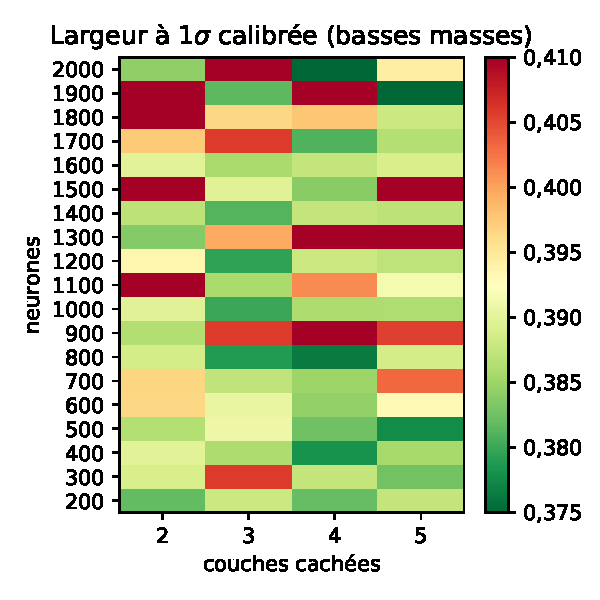
\includegraphics[width=.45\textwidth]{\PhDthesisdir/plots_and_images/my_plots/ML/from_ML_plots/global_comparisons/DNN_structures_all-low_1sig_calibr_width.pdf}

and in the medium mass region we have

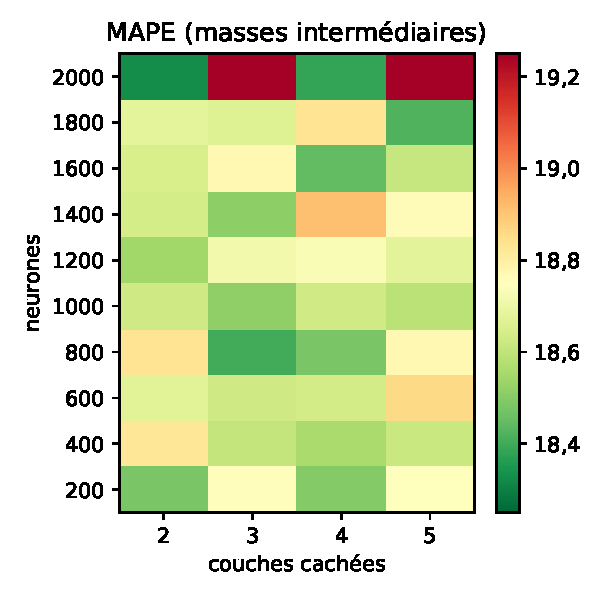
\includegraphics[width=.45\textwidth]{\PhDthesisdir/plots_and_images/my_plots/ML/from_ML_plots/global_comparisons/DNN_structures_reduced-medium_mape.pdf}
%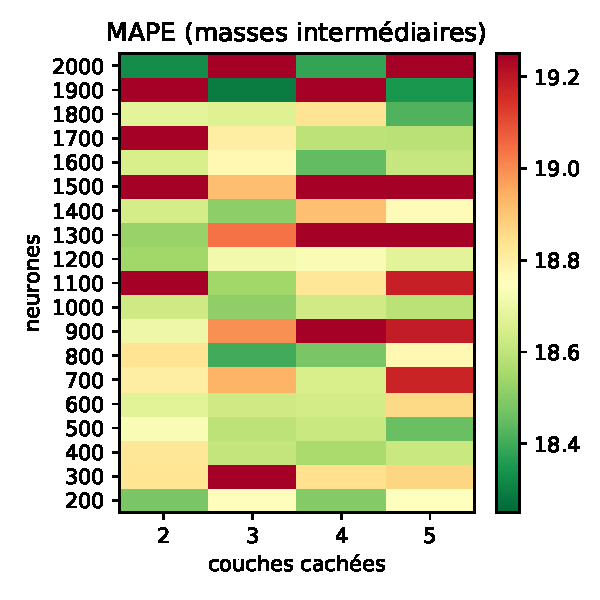
\includegraphics[width=.45\textwidth]{\PhDthesisdir/plots_and_images/my_plots/ML/from_ML_plots/global_comparisons/DNN_structures_all-medium_mape.pdf}

3x1000 is the best compromise we found

\subsection{Fonction d'activation}

activation = softplus

